%======================================================================
\chapter{Valence Bond Entanglement Entropy}
%======================================================================
Recently a new quantity called {\it{valence bond entanglement entropy}} (\vB) was proposed \cite{Ian1, Alet, Chh},  
which seems to have properties similar to the von Neumann entanglement entropy (\vN).
The main advantage of \vb is the simplicity of its measurement when working in the valence bond basis.
For a valence bond basis state \vb between two regions, A and B, it is defined as 
\begin{equation}
\VB_{\rm A} = \ln({2})\mathcal{N}_{\text{A}},
\label{vbeeeq}
\end{equation} 
where $\mathcal{N}_{\text{A}}$ is the number of valence bonds crossing the boundary between
regions A and B.  (See Figure \ref{vbeepic}.)


\begin{figure} {
\includegraphics[width=5in]{./figures/made/presentation/vbee.pdf} 
\centering
\caption[1D Results for \vb with \vn using periodic boundaries]{
The valence bond entanglement entropy \eqref{vbeeeq} between regions A and B of a valence bond basis state is defined as the number of valence bonds crossing between the two regions multiplied by a factor of $\ln(2)$.
This diagram shows a state with $S^{\text{VB}}_{\rm A}= 7 \ln(2)$.
\label{vbeepic}}
} 
\end{figure}


\vb shares some properties with \vN; in particular, for both quantities: $S_{\text{A}} = S_{\text{B}}$.
Also, $\VB = 0$ for systems with no entanglement between regions A and B.
For any single valence bond basis state (not a superposition of valence bond states) \vb and \vn agree exactly.
In one-dimensional Heisenberg spin-1/2 systems \vb seems to to be in good agreement with
results from conformal field theory (CFT) for \vN{} \cite{Alet}.
However, in two dimensions \vb shows a multiplicative logarithmic correction to the area law
for the isotropic Heisenberg model.  
Ground states of unfrustrated 2D spin-1/2 systems with exclusively nearest neighbour interactions
are expected to follow an area law \cite{ALreview, DeBeaudrap2010}, though until now there has been a lack of computational results confirming this.

To examine the correspondence of \vb to a known measure of entanglement  \cite{PRL1} we place our \vb data alongside measurements of \vn
on the same system, calculated with density matrix renormalization group (DMRG) \cite{Scholl05,White92} simulations by I. Gonzalez and R. Melko.
\vb is calculated using a single projector valence bond quantum Monte Carlo (VB QMC) scheme \cite{Sandvik2007, Sandvik_vbqmc}.

In this chapter we begin by looking at the scaling of \vb and \vn for 1D systems with OBC and with PBC, and we compare the value of the conformal charge $c$ to the expected value for this system.
We then attempt to move to 2D, looking at $M$-leg ladder systems to determine the scaling of these entanglement entropies.  

My contribution to this project was the measurement of all of the \vb data using a single projector quantum Monte Carlo program, and I did the linear regression  for the \vb data as well.


%-----------------------------------------------------------------------------------------------------------------------
\section{One Dimensional Systems}
%-----------------------------------------------------------------------------------------------------------------------

\begin{figure} {
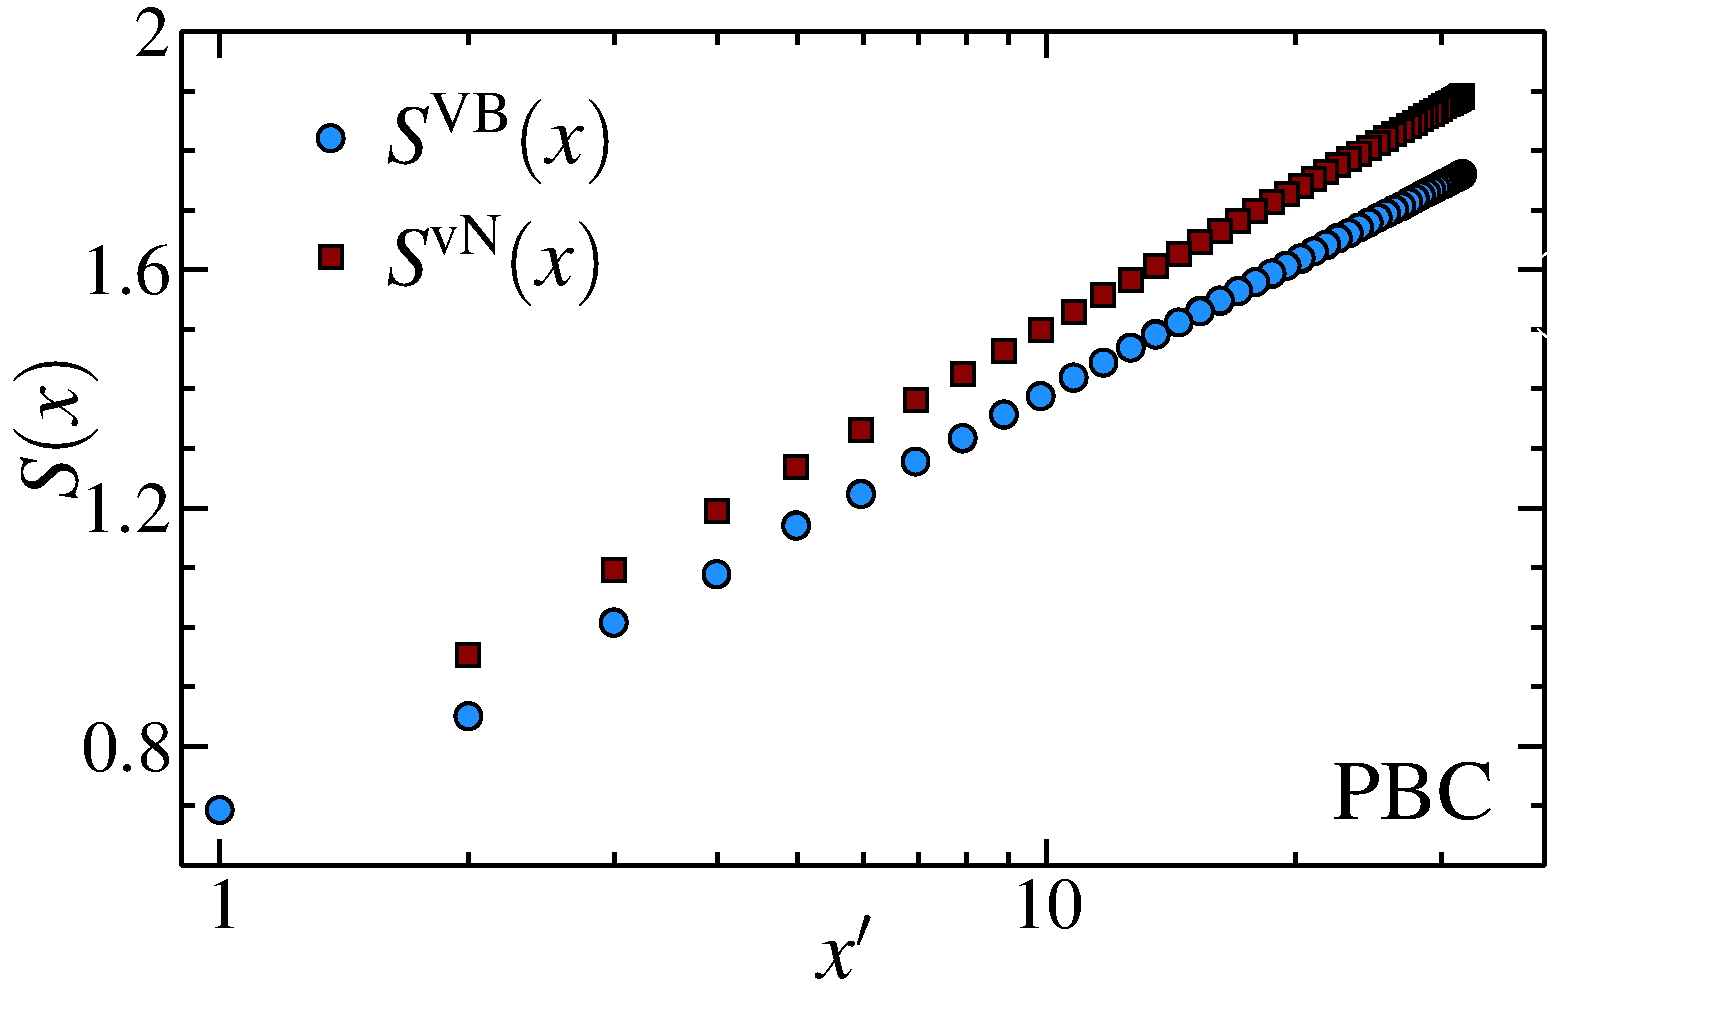
\includegraphics[width=5.5in]{./figures/paper1/figure1/thesis_pbc.pdf} 
\centering
\caption[1D Results for \vb with \vn using periodic boundaries]{
Entanglement entropies for a 1D Heisenberg chain with PBC and L=100 sites, as a function of the conformal distance $x'  = (L/\pi)\sin (\pi x/L)$ \cite{Cardy}.
\label{1dPBC}}
} 
\end{figure}

\begin{figure} 
\vspace{-4cm}
\hspace{3mm}
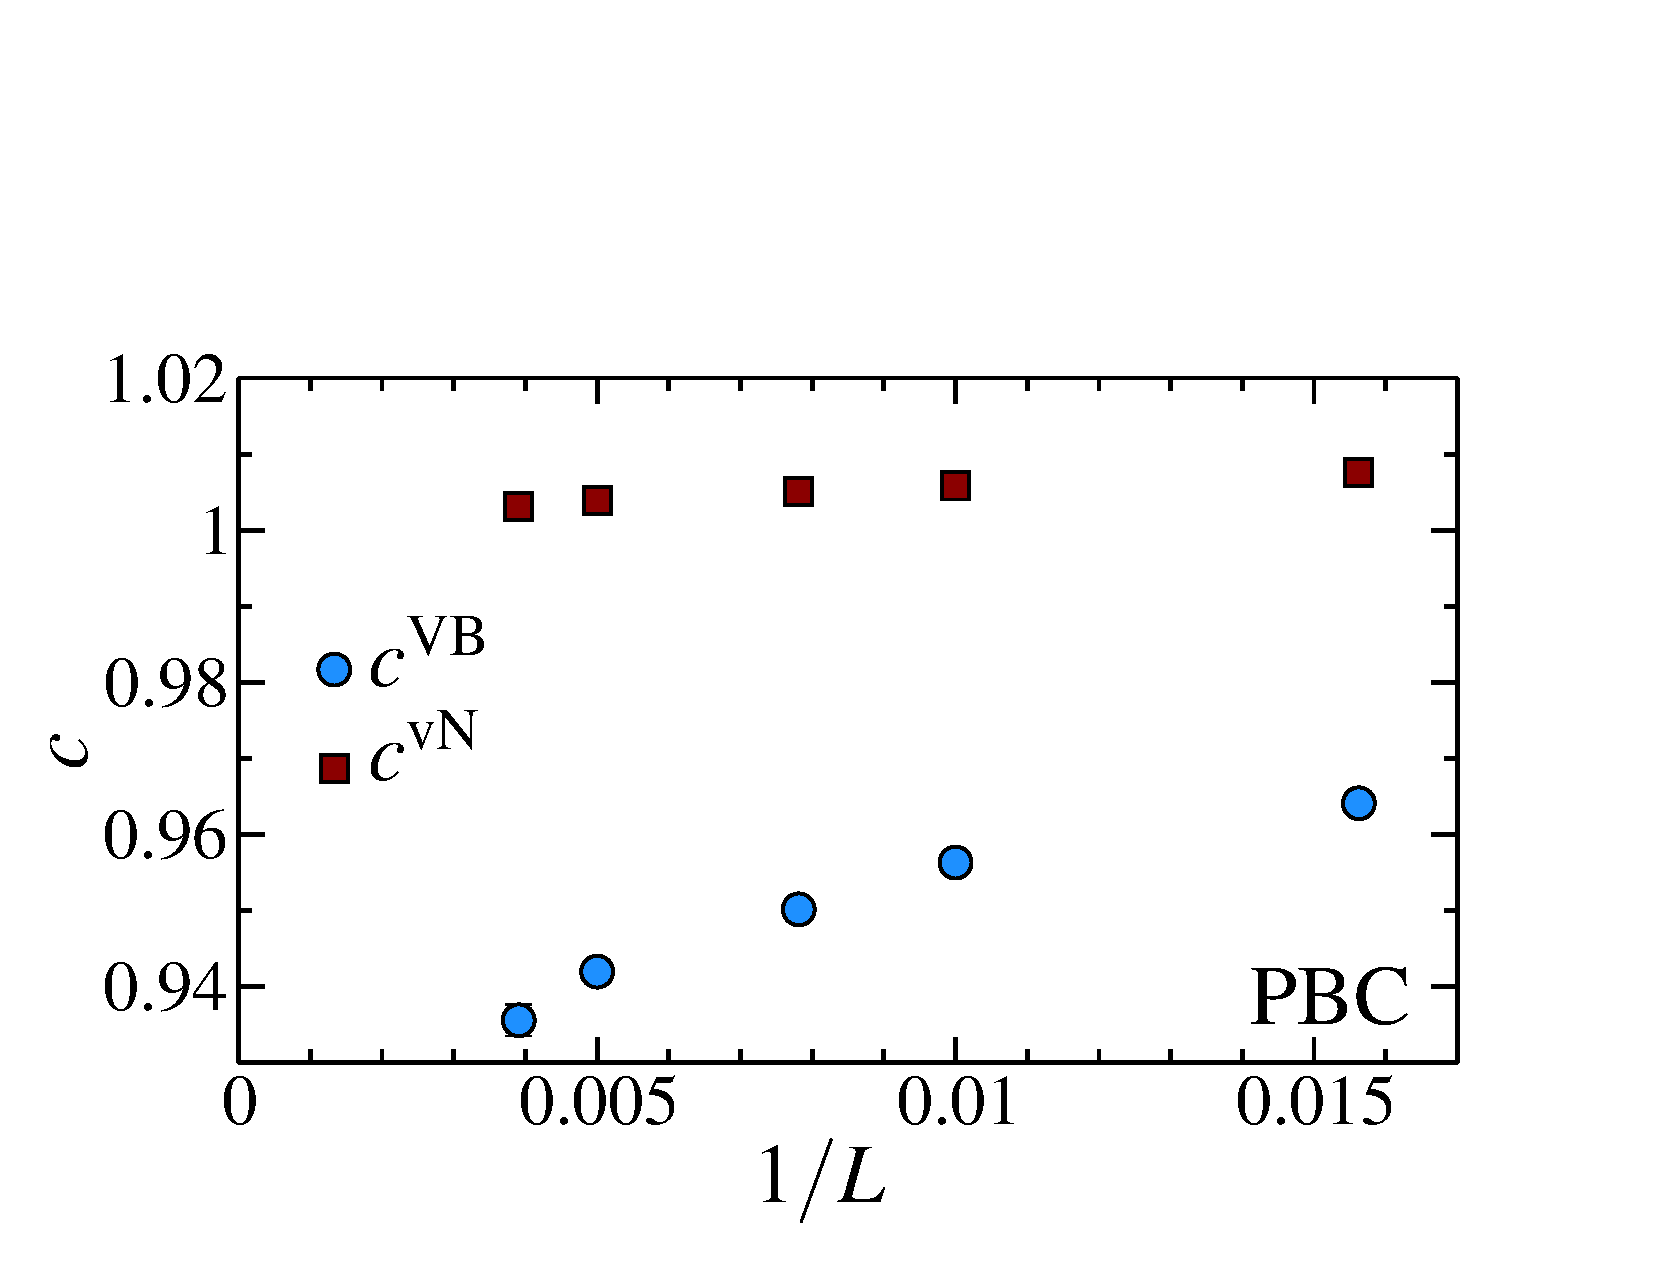
\includegraphics[width=6in]{./figures/paper1/figure1/thesis_c1.pdf} 
\vspace{-4mm}
	\caption[Values of the conformal charge from the 1D periodic boundary results]{
	The central charge, $c$, found using linear regression fits of the entanglement entropy data 	for periodic Heisenberg chains for length L=64, 100, 128, 200, and 256.  Data for the two smallest 	points ($S(1)$ and $S(L-1)$) are removed for the calculation of $c$.
	\label{c1}}
\vspace{1cm}
\hspace{1cm}
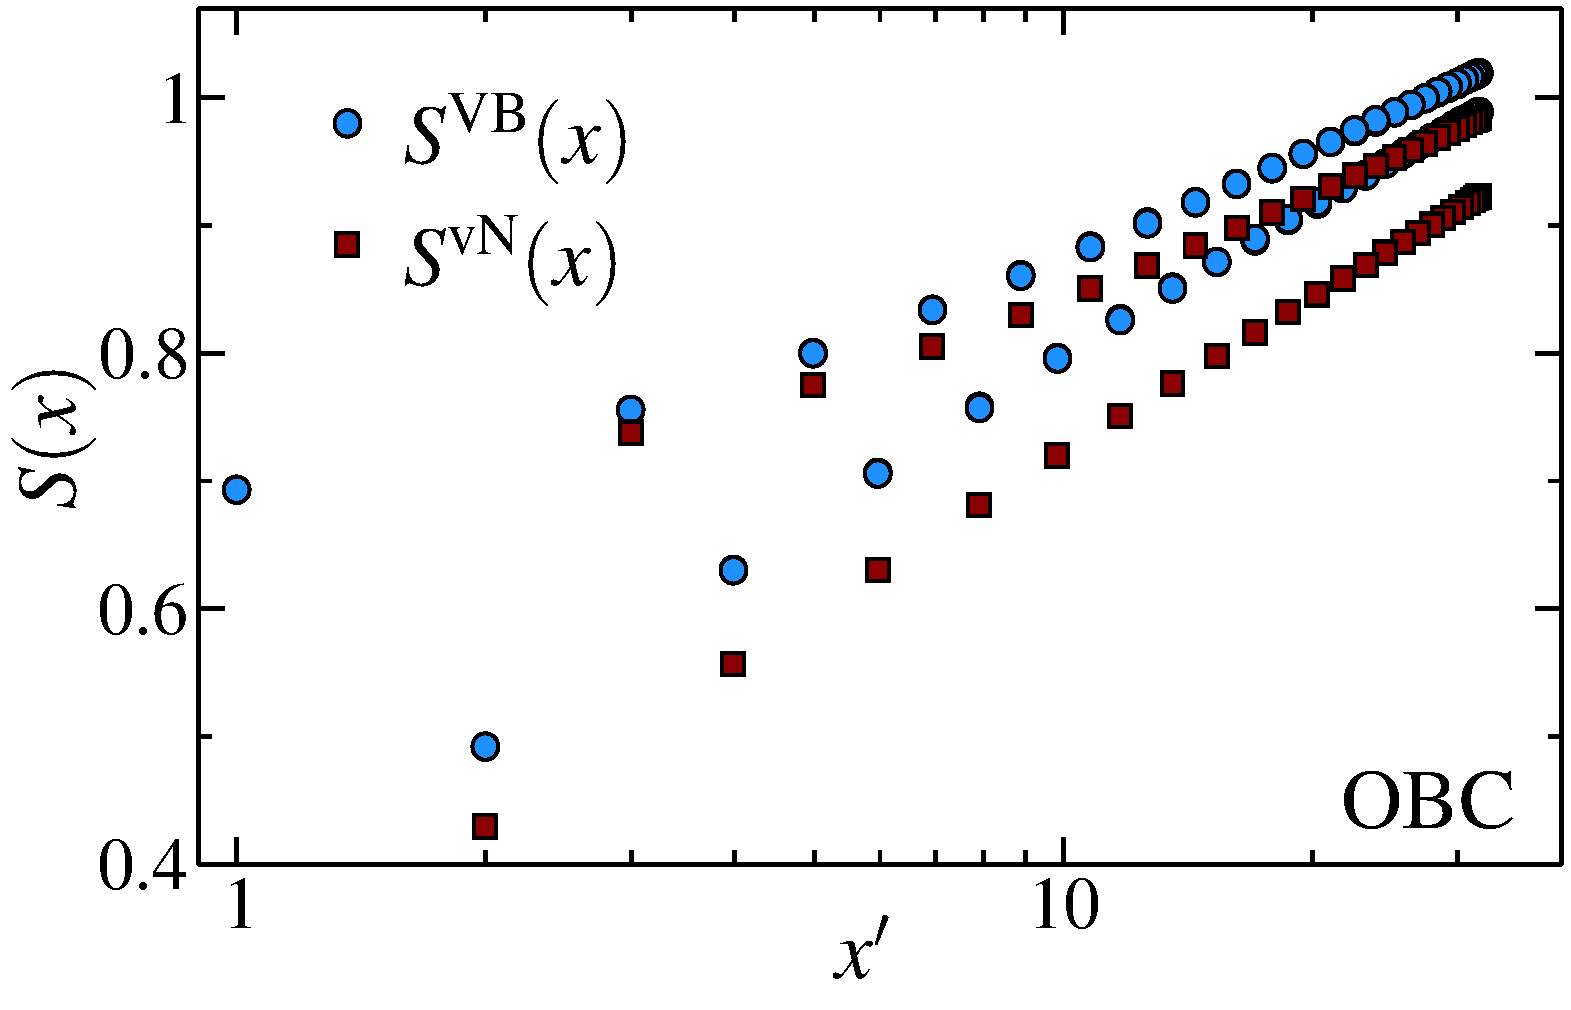
\includegraphics[width=5.1in]{./figures/paper1/figure1/thesis_obc.pdf} 
\caption[1D Results for \vb and \vn using open boundaries]{
	Entanglement entropies for a 1D 100-site Heisenberg chain with OBC as a function of the conformal distance $x'  = (L/\pi)\sin (\pi x/L)$.
	\label{1dOBC}}
\end{figure}


We begin by simulating one dimensional systems, examining both the cases of
open (OBC) and periodic boundary conditions (PBC).
It is convenient to denote the size of region A by the number of sites included in that region 
(i.e. for a 1D system of length $L$, $S_{\text{A}} = S(x)$ is the entanglement entropy for a system where region A contains sites $\{1,2,\dots,x\}$ and the rest of the sites $\{x+1,x+2,\dots,L\}$
belong to region B.

As mentioned in section \ref{1dcft}, for a 1D critical system, such as the 1D Heisenberg spin chain, the scaling of the entanglement entropy is described by  \cite{Cardy, Ian1, Zhou2006}
\begin{align}
	\VN_{\text{PBC}} &= \frac{c}{3}\ln(x') + s_1 \label{cftPBC}\\
	\VN_{\text{OBC}} &= \frac{c}{6}\ln(2x') + \ln(g)+ \frac{s_1}{2} \label{cftOBC}
\end{align}



Figure \ref{1dPBC} shows the \vb measurements for a periodic spin chain of length $L=100$ sites, plotted alongside \vn data.  \vb seems to fit well to the expected scaling, though it is lower than \vN.
We use linear regression to fit the \vb and \vn data for several system sizes to Equation \eqref{cftOBC}, and Figure~\ref{c1} shows the results for the central charge $c^{\rm vN}$ from \eqref{cftOBC} approaching 1 (the expected value for this system \cite{c_is_1}) as the system size increases, however $c^{\rm VB}$ approaches a lower value. 
It has been shown analytically \cite{XXX}, using the probability distribution for valence bonds connecting subsystems of a given length, that $c^{\rm VB} = \tfrac{12\ln2}{\pi^2}\approx 0.84 < c^{\rm vN}$. 



For the 100-site OBC system (Figure~\ref{1dOBC}), we see both \vn and \vb split into two branches, where the upper branch corresponds to an odd number of sites in region A, and the lower branch to an even number of sites.
This branching is due to a ``dimerization" effect caused by the open boundary conditions \cite{Ian1}.
In contrast to the PBC case, \vb is now higher than \vN{} implying that, unlike the successive Renyi entropies, \vb does not give a bound on \vn.
Figure \ref{c2} shows the linear regression fits of the lower branch of OBC data for several different system sizes to Equation \eqref{cftOBC}.  As the number of points included is decreased (until we are only using data where the division between regions A and B is ``far'' from the open boundaries of the system) we see $c^{\rm vN}$ approach a constant value for all system sizes.  As the system size increases $c^{\rm vN}$ approaches the expected value of 1 \cite{c_is_1}.  On the other hand, from the $S^{\rm VB}$ data, it is not clear whether $c^{\rm VB}$ approaches a constant value for large system sizes.  We see only that $c^{\rm VB}$ is lower than the expected value of 1 \cite{Chh}, and that it is lower than the $c^{\rm VB}$ value given by the PBC data.

\begin{figure} {
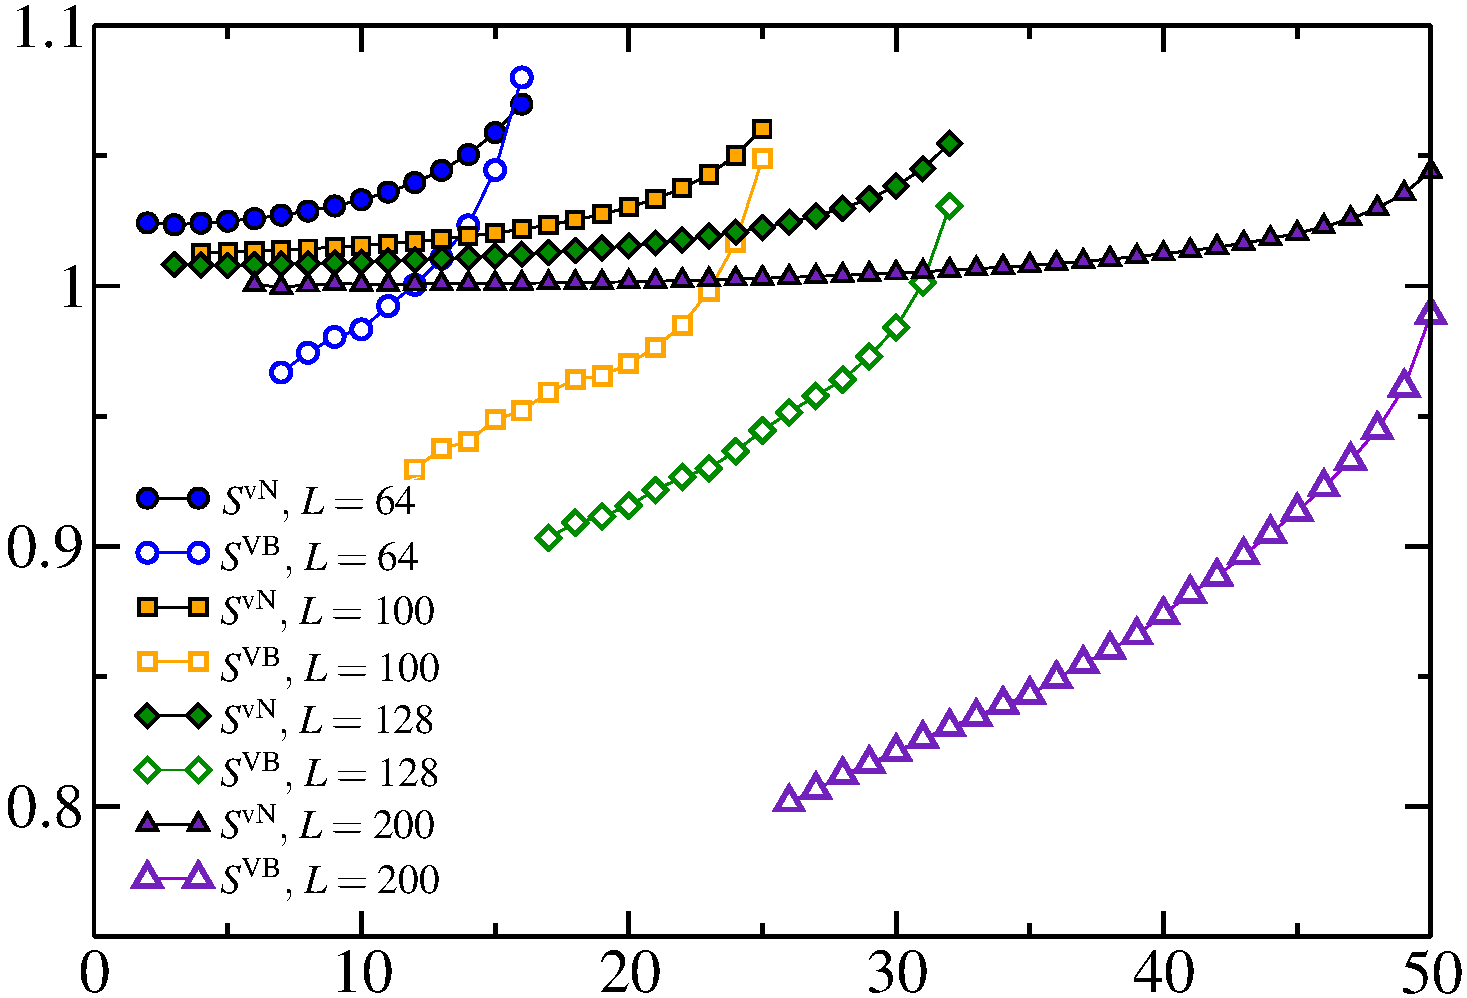
\includegraphics[width=6in]{./figures/paper1/figure1/newfig2.pdf} 
\centering
	\caption[Values of the conformal charge from the 1D open boundary results]{ The central charge, $c$, for 1D OBC chains of lengths $L=64$, 100, 128, and 200.
The slope of the data depends on the number of points $z$ included in the linear regression fit, as can be seen looking at \ref{1dOBC}.
We fit the lower branch of the data, systematically decreasing $z$ until there are too few points left to get an accurate fit.
\label{c2}
}}
\end{figure}


%------------------------------------------------------------------------------------------------------------------
\section{Approaching Two Dimensions}

\begin{figure} { 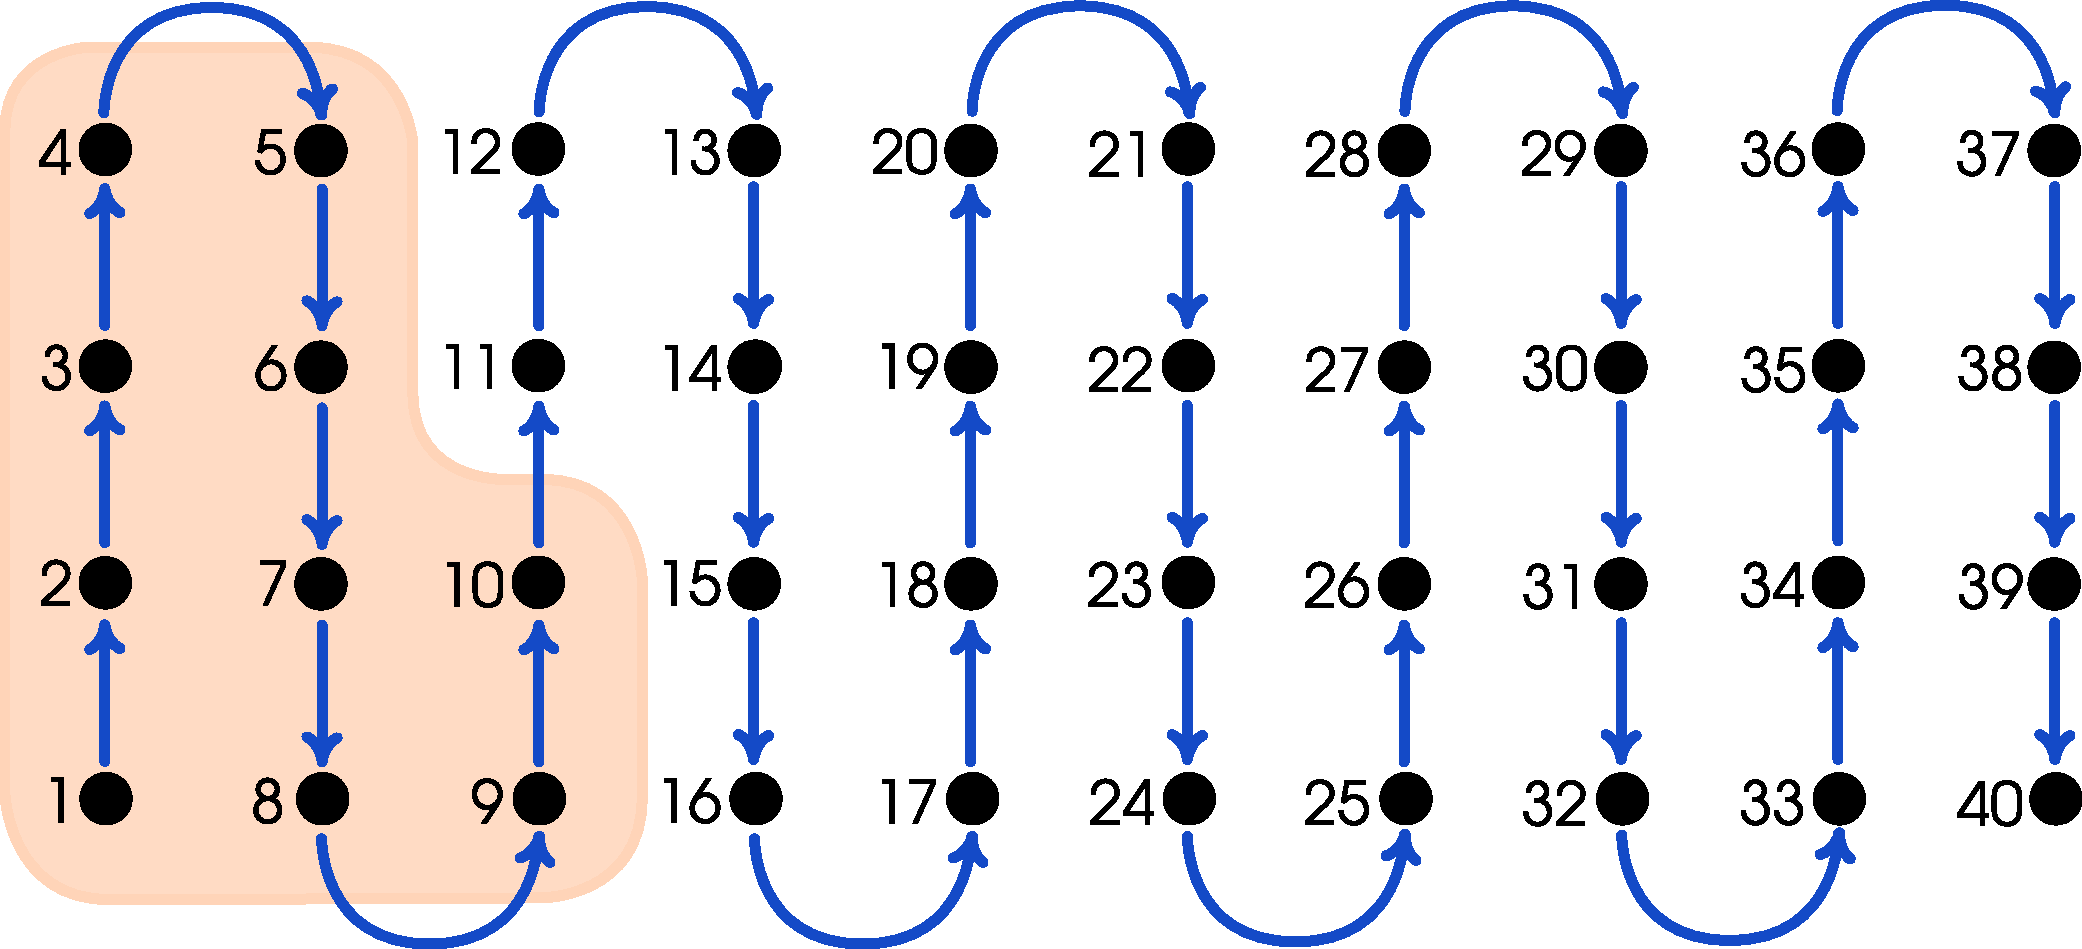
\includegraphics[width=6in]{./figures/made/stuff_covering.pdf}
\centering
\caption[Geometry of a four-leg ladder]{
The site numbering scheme for a $M=4$ leg ladder of length $L=10$.  Region A is the shaded area, and the entanglement entropy of this region is labelled by the largest site $x$ in region A.
In this case $x=10$, and we would measure $S(10)$.  
This geometry is imposed by the DMRG, but we use the same configuration in the VB QMC.
 \label{laddersnake} }} 
 \end{figure}

\begin{figure} { 
\vspace{-1cm}
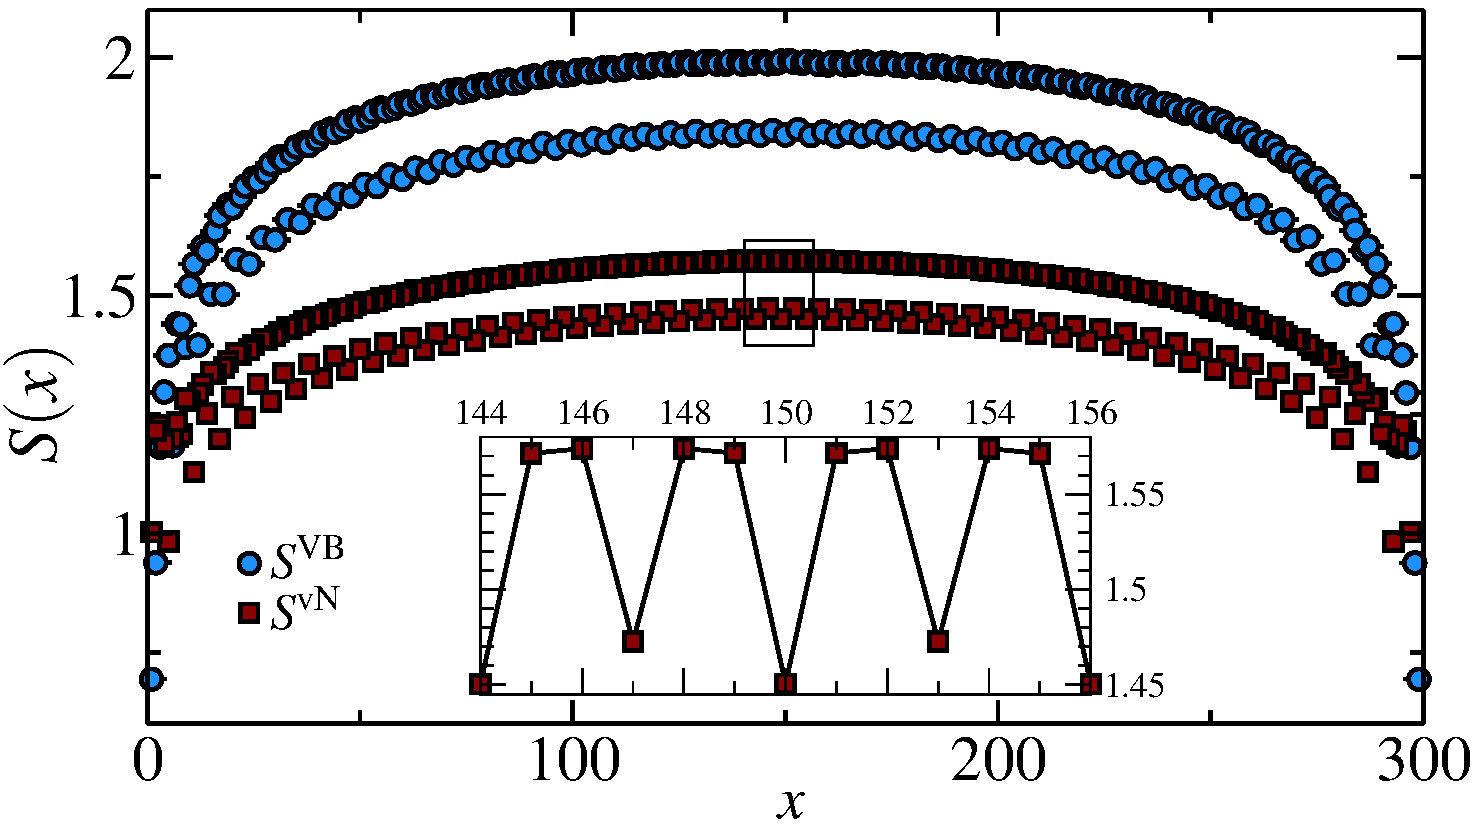
\includegraphics[width=6in]{./figures/paper1/figure3/3-leg-ladder/fig3_final2.pdf}
\caption[Entanglement entropies for a three-leg ladder]{
Entanglement entropies for a three-leg ladder with OBC and 100 sites per leg.  
The inset shows a close up view of the boxed region.
 \label{ladder3} }
 \vspace{1cm}
 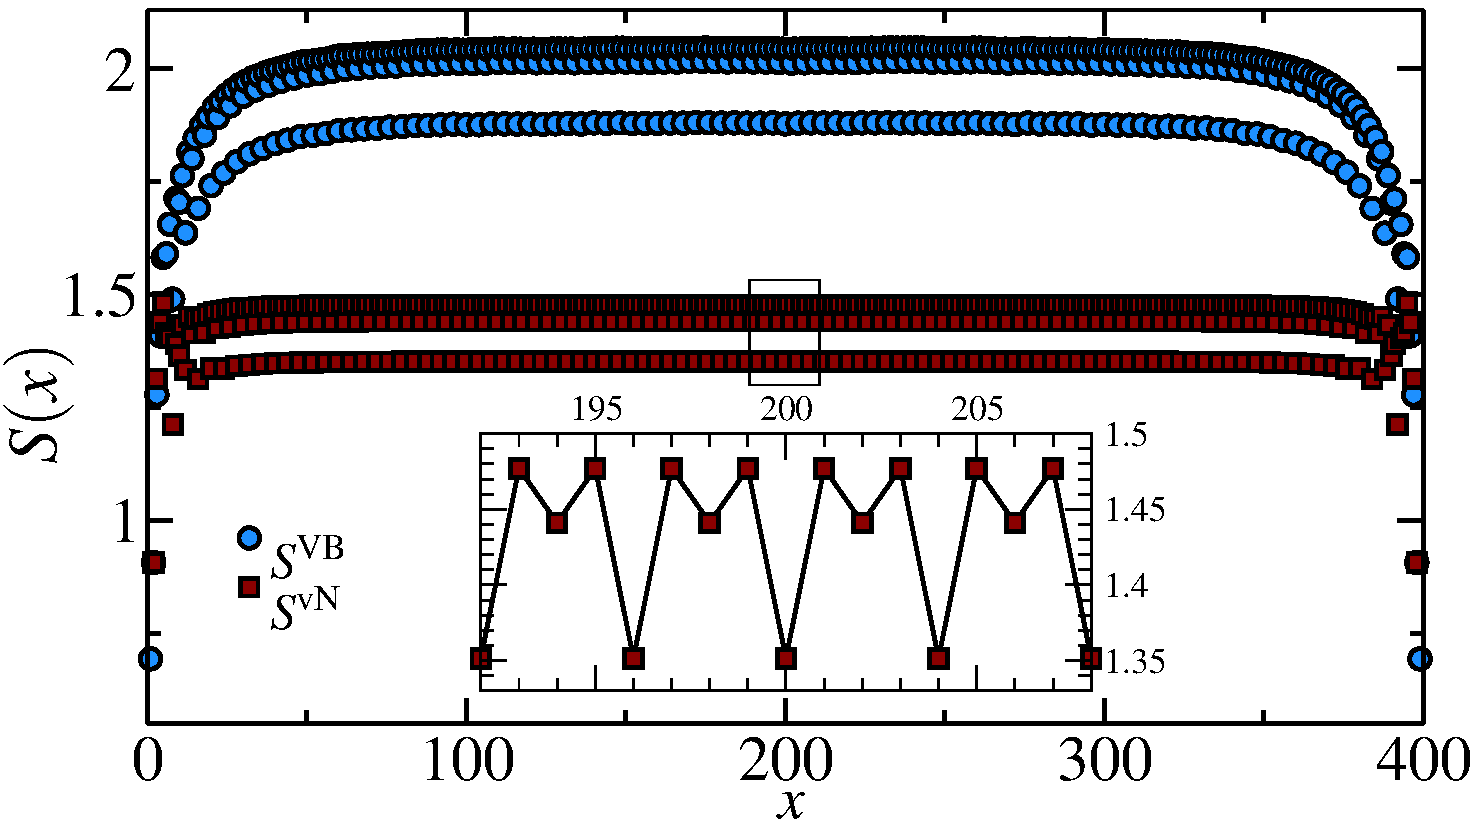
\includegraphics[width=6in]{./figures/paper1/figure3/4-leg-ladder/4legfig.pdf}
\caption[Entanglement entropies for a four-leg ladder]{
Entanglement entropies for a four-leg ladder with OBC and 100 sites per leg.  
The inset shows a close up view of the boxed region.  
 \label{ladder4}}
 
 } 
 \end{figure}
  

 
 We now move towards two dimensions by adding ``legs" to our one dimensional OBC chains.
 Due to the constraints imposed by the DMRG on the geometry of region A the sites must be arranged in a snaking pattern (Fig \ref{laddersnake}).
The DMRG data, to which we compare \vB, are limited to ladders with $M=7$ legs because of the poor scaling of the algorithm when approaching 2D.
 The VB QMC algorithm scales as $Nm$ for a system with N sites \cite{Loops}, so we measure up to $M=20$ with minimal CPU effort.
 
 Figures \ref{ladder3} and \ref{ladder4} show the entanglement entropies for three- and four-leg ladders respectively.
 As with the 1D OBC spin chain, $\VB > \VN$ for these $M$-leg ladders.
 The entanglement entropies show different behavior depending on whether the number of legs is even or odd.
 Odd-leg ladders are gapless, and so all sites contribute to the entanglement, thus
 $S(x) \propto \ln(x')$ as in the 1D case \cite{White1994}.
 Even-leg ladders have a spin gap and so only sites within the correlation length $\xi$ from the boundary between A and B contribute to the entanglement,
so for even-leg ladders $S(x\gtrsim\xi) = \text{const}$. 
Both even- and odd-leg ladders split into branches, as shown in the figure insets, though the even-leg ladders have a pattern with period $M$ whereas the odd-leg ladder entanglement entropies have a period of $2M$.  
 
%------------------------------------------------------------------------------------------------------------------
\section{The Area Law}
\label{vbAlaw}

\begin{figure} { 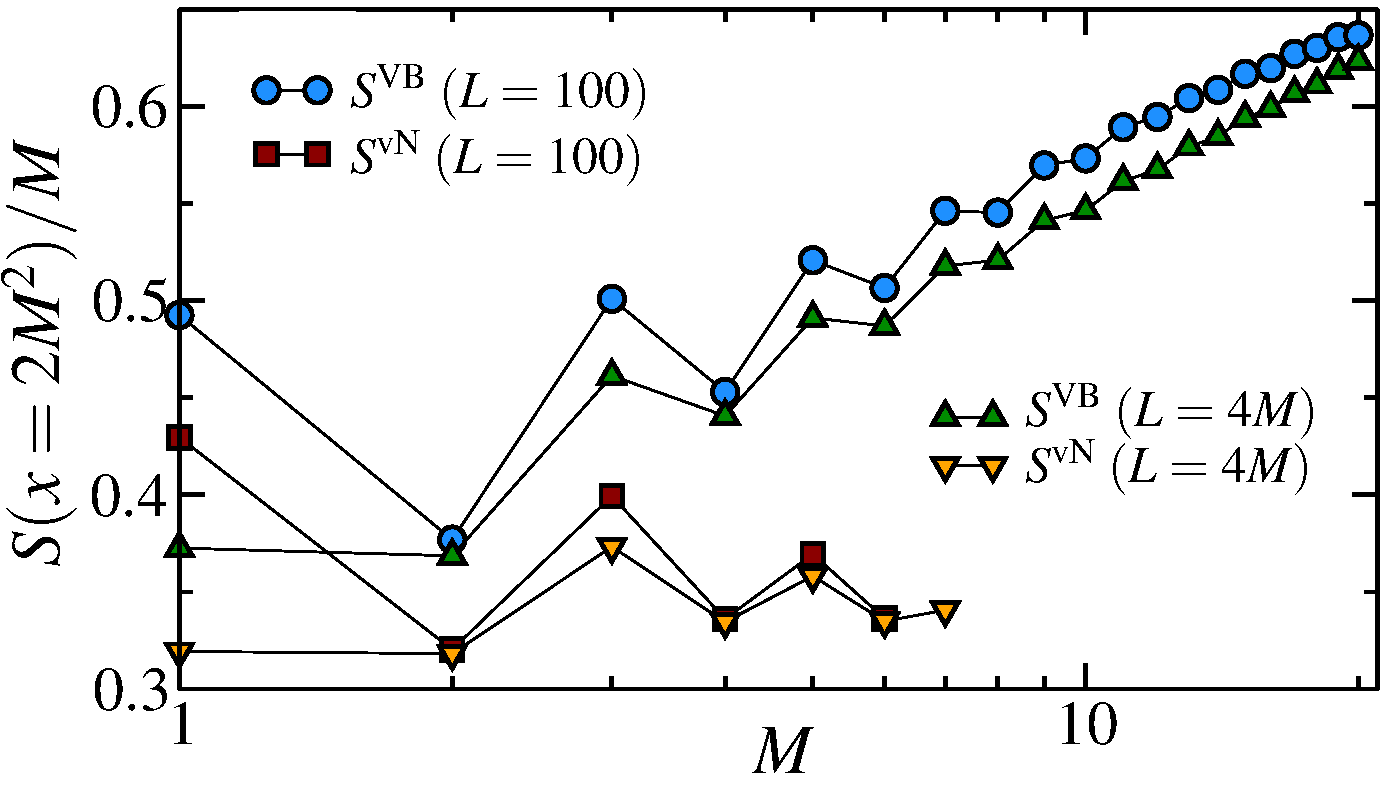
\includegraphics[width=6in]{./figures/paper1/figure4/4fig.pdf}
 \caption[Area law for \vn in 2D Heisenberg ground state, \vb shows a multiplicative logarithmic correction]{
Entanglement entropies divided by $M$,  for $M$-leg ladders, taken such that
the region A includes $2M^2$ sites.  
Data from both ladders of  with $L=100$ sites per leg and ladders of length $L=4M$ 
(with length proportional to the number of legs) are shown.
For large $M$, $S^{\rm VB}\propto M \ln M$,
whereas $S^{\rm vN}\propto M$.   
\label{zigzag}}} 
\end{figure}

Using these multileg ladders we can examine the adherence of the ground state of the 2D isotropic Heisenberg model to the area law.
To do this we use $M$-leg ladders, including $2M^2$ sites within region A.  
This ensures that the boundary between regions A and B cuts cleanly across all the legs of the system so that the length of the boundary is proportional to $M$, while also keeping keeping the dividing line between the two regions far enough from the open boundaries of the system to avoid boundary effects.
Additionally, the 2:1 aspect ratio ensures that, even for odd-leg ladders, an even number of sites is included in region A, reducing the odd-even oscillations in the entanglement entropies.

In Figure \ref{zigzag} we plot the entanglement entropies $S(x)/M$ versus M, for $M$-leg ladders,  on a logarithmic scale.
If the scaling of the entanglement entropy follows an area law we should see $S(x)/M$ approach a constant value for large $M$.
We include both systems with 100 sites per leg, and systems with $4M$ sites per leg. 
In the second case the size of region A is proportional to the size of the ladder, and the dividing line between regions A and B is always cutting the ladder through the middle.

We observe a multiplicative logarithmic correction to the area law in \vB, as previously shown by Refs.\cite{Alet,Chh}.
This correction, however, is not present in the \vn results from DMRG.
\vn convincingly approaches a constant value for large $M$, suggesting that the area law is valid for \vn in the $M \rightarrow \infty$ limit. 
These results also imply that the multiplicative logarithmic correction to the area law (also observed by Alet {\it et al.} \cite{Alet}) is present only in \vB, and not necessarily in all measures of entropy.


%\comment{
%%------------------------------------------------------------------------------------------------------------------
%\section{Bond Length Distribution}
%%------------------------------------------------------------------------------------------------------------------
%We can relate \vb to the bond length distribution $P(x,y)$, defined by Sandvik as the probability of finding a bond between sites $x$ and $y$. 
% Sandvik found that for $P(x,y) \sim \lvert x-y \rvert^{-p}$ with $p \approx 3$ for the \change{2D Heisenberg ground state / N\'eel state}.
%It is possible to relate \vb to the bond length distribution as
%\begin{equation}
%\VB_{\text{A}} = \sum_{x\in \text{A}}\sum_{y\in \text{B}} P(x,y) \ln{(2)}.
%\end{equation}
%\comment{Explain why this gives multiplicative log correction...}
% } 
 
%------------------------------------------------------------------------------------------------------------------
\section{Analytical Calculations}
%------------------------------------------------------------------------------------------------------------------

%\comment{
%There are \change{two} reasons why \vb fails to properly measure entanglement.
%First, linear combinations of valence bond states are not properly normalized, and second, it is possible to have entanglement between two regions even when no valence bond crosses between those regions.
%}


\begin{figure}
\centering
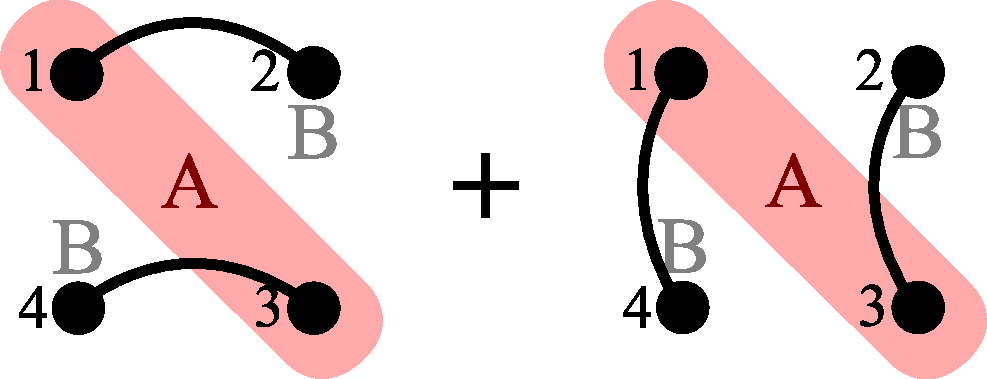
\includegraphics[width=4in]{./figures/made/example1.pdf}
\caption[A superposition of two four-site valence bond states]{An equal superposition of two four-site valence bond states.  
Region A is the shaded region including sites 1 and 4.
Region B contains sites 2 and 3.
For this state $\VB_{\rm A}=2\ln(2)\approx1.386$ and $\VN_{\rm A}=\ln(3)\approx 1.099$.
 \label{example1}
}
\end{figure}

From the 1D results (Figs.~\ref{1dOBC} and \ref{1dPBC}) we saw that \vb can be either greater or less than \vN.
This can be understood through some simple examples, shown in figures \ref{example1} and \ref{example2}.
The first example, Fig.~\ref{example1} is an equal superposition of two four-site valence bond states. 
 \vb is easily calculated as the maximal value, $\VB = 2\ln(2)$, since there are four bonds crossing between regions A and B, and we divide by the number of states (two in this case).
This corresponds to the way \vb would be measured in the single projector VB QMC algorithm.
 For such a small system, it is not difficult to calculate \vn explicitly, and we will do so here.
 We begin by writing out and normalizing the wavefunction in the $S^z$ basis.
 \begin{align}
\hspace{-2mm}
 \ket{\psi} &= C \big[ \left( \ket{\up_1\dw_2} - \ket{\dw_1\up_2}\right) \otimes 
 		\left( \ket{\up_3\dw_4} - \ket{\dw_3\up_4}\right) + 
		\left( \ket{\up_1\dw_4} - \ket{\dw_1\up_4}\right) \otimes 
 		\left( \ket{\up_3\dw_2} - \ket{\dw_3\up_2}\right) \big] \\
		&= C \big[ 2\ket{\up\dw\up\dw} + 2 \ket{\dw\up\dw\up} -
			\ket{\up\dw\dw\up} -\ket{\dw\up\up\dw} - \ket{\up\up\dw\dw} - \ket{\dw\dw\up\up}
			\big] \label{yknow}\\
C &= \frac{1}{\sqrt{\bra{\psi}\psi\rangle}} = \frac{1}{\sqrt{4+4+1+1+1+1}} = \frac{1}{\sqrt{12}}
 \end{align}
 Note that in \eqref{yknow} the spins are in numerical order $\ket{1,2,3,4}$.
 To simplify the process of finding the reduced density matrix $\rho_{\rm A}$ we relabel the states such that
 \begin{eqnarray}
 \ket{\up\up} \rightarrow \ket{a} \hspace{15mm} \ket{\up\dw} \rightarrow \ket{b}  \hspace{15mm} 
 \ket{\dw\up} \rightarrow \ket{c}  \hspace{15mm} \ket{\dw\dw} \rightarrow \ket{d},
 \end{eqnarray}
and a subscript A specifies that the state belongs to spins 1 and 3, while B refers to spins 2 and 4. 
 \begin{eqnarray}
\ket{\psi} = \frac{1}{\sqrt{12}} \big[ 
		2\ket{a}_{\rm A}\otimes \ket{d}_{\rm B} + 
		2\ket{d}_{\rm A}\otimes \ket{a}_{\rm B} 
		- \big(\ket{b} +\ket{c}\big)_{\rm A} \otimes  \ket{c}_{\rm B} 
		 -\big(\ket{c} +\ket{b}\big)_{\rm A} \otimes \ket{b}_{\rm B}
		\big]
 \end{eqnarray}
 When we trace out region B, only the terms that are diagonal in region B will survive. 
  We can avoid writing out the full density matrix and skip straight to the reduced density matrix.
  Now all the states refer to region A, spins 1 and 3.
  \begin{align}
\rho_{\rm A} &=  {\rm Tr_B} \ket{\psi}\bra{\psi} \\ 
		&= \frac{1}{12} \big[ 
		4\ket{a} \bra{a} + 4 \ket{d}\bra{d}
		+ 2\big(\ket{b} +\ket{c}\big)\big(\bra{b} +\bra{c}\big)
		\big] =
		\frac{1}{6}
		\left[ \begin{array}{cccc}
		2 & 0&0&0\\
		0& 1& 1&0\\
		0& 1& 1&0\\
		0& 0& 0&2
		\end{array} \right]
 \end{align}
Diagonalizing $\rho_{\rm A}$ gives three identical eigenvalues of $\tfrac{1}{3}$, which we use to calculate \vN,
\begin{align}
\VN_{\rm A} = - {\rm Tr} \left(\rho_{\rm A} \ln \rho_{\rm A} \right)= -3\left( \frac{1}{3} \ln \left( \frac{1}{3}\right)\right)
		= \ln(3) \approx 1.0986.
\end{align}
For this system (Fig.~\ref{example1}) $\VB =2\ln(2) > \VN \approx 1.0986$.
Though $\VB=\VN$ for non-superpositional valence bond basis states, \vb does not give the correct result for some linear combinations of such states.  

\begin{figure}
\centering 
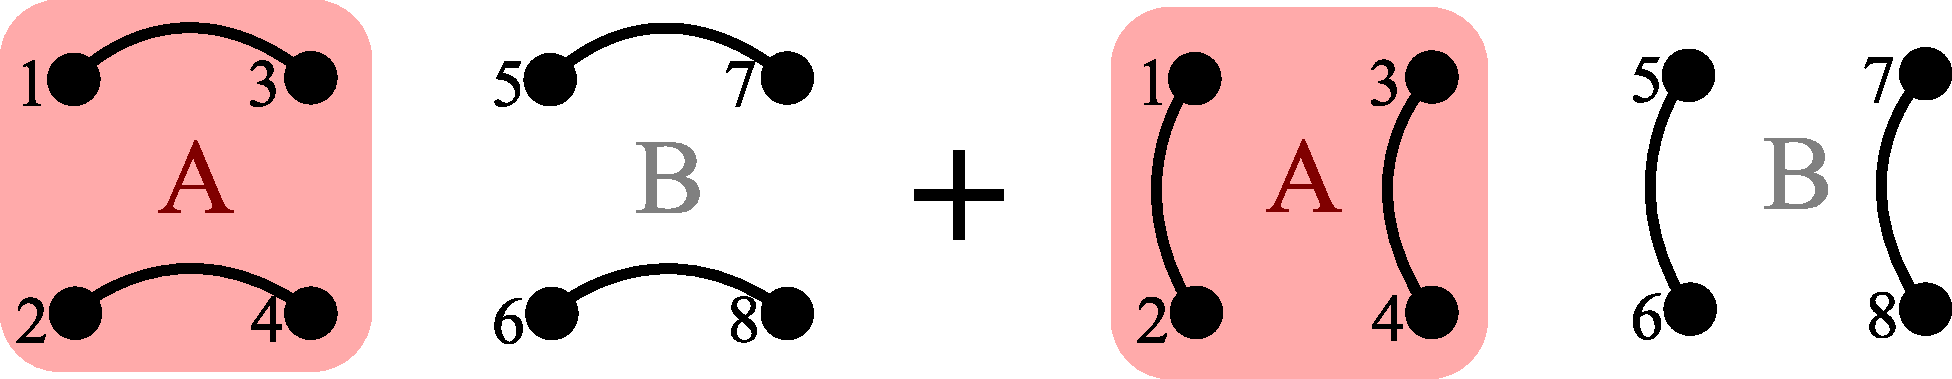
\includegraphics[width=6in]{./figures/made/example2.pdf}
\caption[A superposition of two eight-site valence bond states]{An equal superposition of two eight-site states.
Region A is the shaded region including sites $1-4$.  
Region B contains the remainder of the sites, $5-8$.
For this state $\VB_{\rm A}=0$ and $\VN_{\rm A}\approx 0.325$.
\label{example2}
}
\end{figure}

In Figure \ref{example2} we have another linear combination of states, this time a superposition of two eight-site states, where region A includes the four sites on the left-hand side.  In this case we find that \vb underestimates \vn since there are no valence bonds crossing between regions A and B, but the two regions are still entangled.  The calculation of \vn for this state can be seen in Appendix~\ref{small}, where we find $\VN\approx 0.3251$.



%------------------------------------------------------------------------------------------------------------------
\section{Discussion}
%------------------------------------------------------------------------------------------------------------------

We have compared the scaling properties of the valence bond entanglement entropy \vb \cite{Alet,Chh}, to the von Neumann entanglement entropy \vn in the spin-1/2 Heisenberg model in 1D and on multi-leg ladder systems, using both VB QMC and DMRG simulations methods.
In 1D, we find that \vb closely follows the behavior of \vN, though it is less than \vn for periodic chains, and greater than  \vn for chains with open boundaries.

We also fit both entanglement entropies to the 1D conformal field theory results (Eqs.\eqref{cftPBC} and \eqref{cftPBC}), which show excellent agreement for \vN, but show significant deviation from the expected value of $c$ for \vb in the large chain length limit, approaching $c<1$ for both open and periodic boundary conditions \cite{XXX}.

We then examined $M$-leg ladder systems, cutting across all legs such that the boundary size scales with the number of legs, where we see from the DMRG results that \vn obeys the area law in the many-leg limit.  
On the other hand, \vb has a multiplicative logarithmic correction to the area law for the N\'eel ground state.
This correction may be due to the fact that \vb is not well-defined for a superposition of valence bond basis states.  In general, for some valence bond basis states $\psi_1$ and $\psi_2$, $\VN(\psi_1 + \psi_2) \ne \VN(\psi_1) + \VN(\psi_2)$, however we use  $\VB(\psi_1 + \psi_2) = \VB(\psi_1) + \VB(\psi_2)$ to get the valence bond entanglement entropy

%To help understand the discrepancy between these two measures of entanglement, we show simple examples of a system with $\VB > \VN$ (Fig. \ref{example1}) and a system with $\VB > \VN$ (Fig. \ref{example2}).  
%\comment{say something else.}

While it is clear that \vb is a reasonable measure of entanglement, easily accessible to scalable numerical simulations, the inability of this quantity to provide a bound on \vN{}, unlike other measures of of entanglement entropy, together with its multiplicative logarithmic correction to the area law in 2D make \vb less suitable for characterizing topological phases, or studying universal quantities at quantum phase transitions.

In the next chapter we explore an alternative method for measuring entanglement in large-scale quantum Monte Carlo simulations.












